\documentclass{article}
\usepackage{enumitem}
\usepackage{indentfirst}
\usepackage{amsfonts}
\usepackage{hyperref}           % Use links
\usepackage{graphicx}           % Coloque figuras
\usepackage{float}              % [...] no lugar adequado!
\usepackage[T1]{fontenc}        % Encoding para português 
\usepackage{lmodern}            % Conserta a fonte para PT
\usepackage[portuguese]{babel}  % Português
\usepackage{hyphenat}           % Use hifens corretamente

\graphicspath{{./img/}}

\hyphenation{mate-mática recu-perar}

\setlist{  
    listparindent=\parindent,
    parsep=0pt,
}

\def\code#1{\texttt{#1}}

\author{\textbf{Igor Lacerda Faria da Silva\( ^1 \)} }

\title{\textbf{Trabalho Prático 1}

\textbf{Escalonador de URLs}}

\date{%
    \( ^1 \)Departamento de Ciência da Computação - Universidade Federal de Minas Gerais (UFMG) - Belo Horizonte - MG - Brasil \\ [2ex]
    \href{mailto:igorlfs@ufmg.br}{\nolinkurl{igorlfs@ufmg.br}}
}

\begin{document}

\maketitle

\section{Introdução}

O problema proposto foi implementar um escalonador de URLs, como parte de um coletor de uma máquina-de-busca. O propósito de um escalonador é auxiliar na definição de uma ordem para que as páginas sejam coletadas. Existem diversas estratégias para realizar essa tarefa, mas a adotada nesse trabalho foi a \textit{depth-first}, que consiste em coletar todas as URLs de um dado host antes de passar para o próximo. Foi implementada uma leitura de arquivos, que continham uma série de instruções para a execução do escalonamento, cuja saída também foi impressa em um arquivo.

Esta documentação tem como proposta explicar como se deu essa implementação, desde questões mais ligadas ao funcionamento do programa (Seção 2) e estratégias de robustez (Seção 4) como análises de complexidade (Seção 3) e experimentais (Seção 5). Ao final do texto, encontra-se uma conclusão (cujo conteúdo está mais relacionado ao aprendizado pessoal do autor com o trabalho), bibliografias e, por último, as instruções para compilação e execução.

\section{Método}

O programa foi desenvolvido em C++ e compilado utilizando o g++, do GNU Compiler Collection. A máquina que foi usada durante o desenvolvimento conta com 3.8Gi de memória RAM, e processador Intel(R) Core(TM) i3-2350M CPU @ 2.30GHz, e roda o sistema operacional GNU/Linux (versão do kernel: 5.15.6).

A formatação do código fonte (\textbf{incluindo a indentação}): \textbf{foi feita usando a ferramenta clang-format}. Foi usado um arquivo customizado para isso, que se encontra na raiz do projeto, com o nome de \textit{.clang-format}. É um arquivo bem curto, baseado em preferências pessoais do autor, mas que \textbf{garante a consistência da formatação do projeto}.

Ambos os desafios foram implementados. Foi usado o \code{git} para controle de versão, então, para cada desafio optou-se por criar uma \textit{branch}, modificando as funções já implementadas na estratégia padrão (além da criação de métodos e membros auxiliares). Assim, as estratégias estão separadas por nome na raiz da pasta de entrega. Para mais detalhes, solicite acesso ao \textit{repo} no Github.

\subsection{Organização do código}

O projeto atende à especificação no que diz respeito à organização do código de forma geral (cabeçalhos em \code{./include}, etc). Em particular, a única divergência é que os \emph{headers} usam a extensão \code{.hpp} e não \code{.h} (idiossincrasia do editor de texto).

Alguns dos arquivos de cabeçalho definem estruturas de dados mais básicas e gerais, como \code{cell.hpp}, que define uma célula genérica de lista usando templates; \code{linearlist.hpp}, que define uma lista abstrata; e 2 especializações baseadas em alocação dinâmica de memória, a saber \code{linkedlist.hpp} (lista encadeada) e \code{linkedqueue.hpp} (fila encadeada). Outros arquivos já apresentam estruturas mais voltadas à aplicação em questão, como \code{url.hpp} (um conjunto de strings conforme definido na especificação), \code{site.hpp} (um Host e uma lista de de URLs, para serem os membros da fila) e \code{escalonador.hpp}, que implementa de fato as diversas operações solicitadas. Por fim, também tem os ligados à robustez e às análises, como o \code{msgassert.hpp}.

A estruturas dos arquivos fonte é similar, mas algumas classes possuem métodos muito simples, que não foram implementados num arquivo fonte separado. As listas não abstratas e a classes \code{URL}  e \code{Escalonador} foram implementados separadamente. O último arquivo dessa categoria é o programa principal, que se limita a fazer somente o básico para atender à especificação, chamando métodos implementados em outras partes do programa.

\subsection{Estruturas de Dados, TADs e métodos}

Existem duas estruturas de dados principais no programa: lista encadeada e fila (encadeada). Ambas são derivações de uma estrutura \textit{lista linear}, sendo que a fila é muito mais restritiva com relação a algumas operações, como inserção e remoção. Em princípio, a lista linear consiste numa sequência de \( n \) elementos (que pode ser vazia), em que há noção de sucessão e antecedência. Nesse sentido, uma propriedade interessante é a existência de um elemento que não tem sucessores (chamado cauda) e um elemento que não tem antecessores (chamado cabeça), que não são necessariamente distintos.

Neste trabalho, uma classe abstrata \code{LinearList} foi usada para representar uma lista linear. Ela possui apenas um membro, \code{size} (int), e métodos muito simples: um construtor que inicializa o membro como 0, um método \code{getSize()}  que retorna \code{size}, um método \code{empty()} que verifica se \code{size} é igual a 0, e um método virtual de limpeza: \code{clear()}.

\subsubsection{Lista Encadeada}

A primeira especialização de lista linear trabalhada foi a lista (simplesmente) encadeada, implementada na classe \code{LinkedList} (herdeira de \code{LinearList}). Na lista simplesmente encadeada, cada elemento é uma célula, que possui seu conteúdo e um apontador para a posição seguinte. A célula foi implementada na classe \code{Cell}, que possui esses membros e um construtor que inicializa a posição seguinte para nulo. A \code{LinkedList} usa alocação dinâmica de memória, com uma célula cabeça cujo conteúdo não importa, tendo como propósito simplificar a implementação de alguns métodos, e células do tipo \code{URL}.

A implementação da classe \code{LinkedList} teve como grande inspiração as aulas do professor Chaimowicz. Os principais métodos são os de construção, destruição (e limpeza), inserção e remoção. No construtor somente é criada uma nova célula, que assume o papel de cabeça e cauda. No destrutor, o método auxiliar \code{clear()} é chamado, e a célula restante é destruída. O método \code{clear()} deleta as células em sequência, caso existam. Há 2 métodos de inserção, a depender da posição: \code{insertBeg()}, para o começo e \code{insertPos()} em uma posição arbitrária. A classe também conta com um método de remoção, \code{removeBeg()}, que remove elementos do começo (não foi preciso remover elementos de outras posições, pela especificação).

Além disso, há um método de impressão \code{print()} (que imprime, em sequência, as URLs) e alguns voltados para o uso com URLs: o \code{searchDepth()}, que compara as profundidades das URLs para definir a posição de inserção (que é em seguida passada para o \code{setPos()}) e o \code{containsUrl()} que verifica se uma dada URL está presente na lista. Por fim, existem dois métodos de escalonamento: um que toma um inteiro \( n \) como parâmetro, e escalona até \( n \) células, e um que escalona toda a lista.

\subsubsection{Fila Encadeada}

Em filas, que são um tipo específico de listas, a inserção só é permitida em uma extremidade e a remoção só é permitida na outra extremidade. Na classe \code{LinkedQueue} (herdeira de \code{LinearList}), que implementa uma fila, a inserção só é permitida nos fundos (\textit{rear}) e a remoção então só é permitida na frente (\textit{front}). De resto, ela é semelhante à \code{LinkedList}, também inspirada nas aulas do professor Chaimowicz, fazendo uso de células e afins. Em particular, ela é uma fila de Sites (tipo \code{Site}), que é uma classe que contém um Host e uma lista de URLs. Os principais métodos da \code{LinkedQueue} são o contrutor, destrutor (e limpar), enfileirar (\code{line()}), que funcionam de forma semelhante aos seus análogos da \code{LinkedList} (aqui, \code{line()} é como \code{insertBeg()}, já que é a única posição permitida de inserção).

Ademais, também possui métodos relacionados ao uso do escalonador em si, como o método que retorna a lista de URLs dado um Host (se estiver presente) (\code{getUrlsFromHost()}), e duas funções de impressão distintas (uma imprime os Hosts e a outra imprime até \( n \) URLs entre todas da fila, em ordem). Finalmente, o método \code{escalonaTudo()}, que chama o método de escalonar tudo para cada um dos sites da fila.

\subsection{Outras classes}

Além das listas (e célula), o programa conta com 3 classes ligadas ao escalonamento: \code{URL}, \code{Site} e \code{Escalonador}. A \code{URL} é somente um conjunto de strings, cada uma representando uma parte da URL (protocolo, host, path, etc), um natural (a profundiade), e alguns métodos: diversos \textit{getters}, um método de impressão (\code{print}) e 2 contrutores, um \textit{default} (necessário para o uso como célula via templates) e um que constrói uma URL dada uma string. Essa classe foi implementada para simplificar alguns requisitos na construção de URLs e facilitar a separação entre as diferentes partes da URL.

A classe \code{Site}, como mencionado anteriormente, tem como propósito fundamental aliar uma lista de URLs a um Host (string), possuindo alguns \textit{getters}, \textit{setters}, \textit{printers}\footnote{Achei essa terminoliga apropriada para métodos de impressão.} e 2 construtores: um \textit{default} e um que dada uma URL, inicializa o Host e a cabeça da lista de URLs. O interessante dessa implementação é que ela permite separar os Hosts da sua lista de URLs, assim, é possível escalonar e continuar ``lembrando'' do Host.

A classe \code{Escalonador} possui como membros uma fila de sites e um arquivo de saída, e implementa todos os métodos da especificação, além de alguns adicionais, para a leitura do arquivo (\code{readFile()}) e auxiliar durante a inserção (\code{addUrls(), isUrlForbidden()}). E claro, um destrutor e um contrutor, que manejam o arquivo de saída.

\section{Análise de Complexidade}

A seguir, são analisadas as complexidades de tempo e de espaço dos principais métodos (as 8 instruções da especificação) do escalonador. A escolha de analisar somente esses métodos teve como base \href{https://virtual.ufmg.br/20212/mod/forum/discuss.php?d=31528}{\nolinkurl{essa}} pergunta do fórum. Alguns pressupostos foram tomados, como assumir que certas funções padrões de C++ são \(\Theta(1)\). Outra presunção é que o construtor de URLs com parâmetro é \( \Theta(1) \), o que não é bem verdade.

\subsection{Métodos}

\begin{itemize}

    \item ADD\_URLS (\code{addUrls()} e \code{insertUrl()})

        \textbf{Tempo:} a inserção de URLs é dividida em 2 métodos. \code{addUrls()} tem finalidades simples: coletar a linha, verificar se o final do arquivo foi atingido e chamar \code{insertUrl()} se a linha coletada for válida. \code{insertUrl()} é o ``cérebro'' da inserção. Por isso, não vou analisar minuciosamente \code{addUrls()}. São realizadas algumas verificações para a inserção, e algumas declarações de variáveis do tipo string, todas \( O(1) \). Em seguida, é usada a função \code{getUrlsFromHost()}. Essa função aparece em diversos métodos. Ela busca na fila, sequencialmente, se dado Host está presente, e se estiver, retorna sua lista de URLs (caso contrário um ponteiro nulo é retornado). Para \code{insertUrl()}, o melhor caso é se o Host está ausente, pois aí a fila é estendida, e o método para enfileirar é \( \Theta(1) \). Então, no melhor caso, a inserção é \( \Theta(n) \), para \( n \) tamanho da fila. 

        Se o Host está presente, existe variação conforme a posição na fila (se o Host corresponde ao primeiro elemento, temos o melhor caso, se corresponde ao último, temos o pior), e deve ser avaliado se a URL já foi inserida anteriormente. Se a URL for repetida, nada é realizado. Mas para se verificar que a URL é repetida, é preciso conferir, o que é \( \Theta(m) \), pela busca sequencial de \code{containsUrl()}. Considerando o pior caso, temos \( \Theta(n+m) \) nessa situação. Mais uma possibilidade é \textit{Host presente, URL ausente}: a princípio é recuperada a \textit{profundidade} da URL em tempo constante, é feita uma busca para encontrar a posição certa de inserção (que na pior das hipóteses é a última), e por úlitmo, a inserção na posição correta, com \code{insertPos()}, que chama \code{setPos()}. Então, recapitulando o pior cenário possível: Host presente, URL ausente, URL tem profundidade maior do que as presentes. Assim, além das buscas supracitadas, \code{searchDepth()} e \code{insertPos()} ``adiconam um nível à linearidade'' (ambos \( \Theta(m) \)), cada, concluindo \( \Theta(n +3m) \). Aqui com certeza existe uma redundância, entre a busca pela profundidade correta e a inserção, que caminha até a posição correta.

        \textbf{Espaço:} com Host ausente ou URL repetida, esse método é \( \Theta(1) \) com relação a complexidade de espaço. Nos outros casos também, nenhuma estrutura depende de algum tamanho em particular.

    \item ESCALONA\_TUDO (\code{escalonaTudo()})

        \textbf{Tempo:} essa função chama \code{escalonaTudo()} da classe \code{LinkedQueue}, que por sua vez faz chamadas sucessivas à função \code{escalonaTudo()} da classe \code{LinkedList}, e uma verificação \( O(1) \). A fila é percorrida completamente, supondo-se tamanho \( n \). No método da lista, cada uma é percorrida \( m_i \) vezes, em que \( m_i \) é o tamanho de cada lista. Certamente existe uma lista com \( M \) elementos tal que \( M \geq m_i \forall i \mid 1 \leq i \leq n \). No pior dos casos é possível então assumir que todas as listas têm tamanho \( M \). Então, cada elemento da fila entra em um laço que é executado \( M \) vezes. Assim, temos que a complexidade assintótica de tempo do método \code{escalonaTudo()} é \( \Theta(Mn) \), ou seja, quadrática. Também podem ser consideradas outras situações, como: todos os Sites \textit{estão vazios.} Nesse caso, o \code{escalonaTudo()} da lista só executa uma comparação, então nesse caso o método como um todo fica \( \Omega(n) \).

        \textbf{Espaço:} apesar de existirem múltiplos casos, todos envolvem estruturas auxiliares unitárias, então a complexidade de espaço é \( \Theta(1) \).

    \item ESCALONA (\code{escalonaN()})

        \textbf{Tempo:} essa função chama \code{escanolaNUrls()} da classe \code{LinkedQueue} e faz uma verificação. Se a fila não está vazia, são executados dois laços \textit{nestados}. No laço de fora, são realizadas operações de custo constante. No laço de dentro também! A remoção do começo e a impressão só envolvem operações unitárias. A regra que quebra ambos os laços está relacionada a \( n \), parâmetro da função. Desse modo, apesar de o laço interior também ser controlado pelo tamanho da lista de URLs de um dado Site, a função \code{escalonaNUrls()} como um todo não tem complexidade quadrática\footnote{Pelo menos essa é minha hipótese, que \href{https://virtual.ufmg.br/20212/mod/forum/discuss.php?d=32885}{\nolinkurl{postei}} no fórum e na véspera da data de entrega ainda não foi confirmada por algum monitor ou professor.}. De fato, se \( n \) é maior que a quantidade de URLs na fila como um todo, a execução é parada ao se atingir o fim da fila, ou seja, a complexidade de tempo da função é \( \Theta(k) \), em que \( k \) é a quantidade de URLs na fila.

        \textbf{Espaço:} são criadas diversas estruturas auxiliares de tamanho constante. Portanto, a complexidade de espaço é \( \Theta(1) \).

    \item ESCALONA\_HOST (\code{escalonaHost()})

        \textbf{Tempo:} essa função chama \code{getUrlsFromHost()}, e caso o Host esteja presente, escalona-o. Se o Host estiver ausente, a fila inteira é caminhada, em complexidade \( \Theta(n) \), em que \( n \) é o tamanho da fila, mas há um retorno logo em seguida. Se o Host estiver na fila, o melhor caso é se ele corresponder ao primeiro elemento da fila, e o pior é se ele corresponder ao último. É feita uma verficação do parâmetro \code{int} passado: o escalonamento só ocorre para, no máximo \( k \) elementos, em que \( k \) é o tamanho da lista. Ou seja, se supormos um parâmetro arbitrariamente grande, o laço será executado ainda \( k \) vezes. Desse modo, no pior caso, considerando a busca inicial, esse método tem complexidade de tempo \( \Theta(n+k) \).

        \textbf{Espaço:} são criadas algumas estruturas auxiliares unitárias. A complexidade de espaço é \( \Theta(1) \).

    \item VER\_HOST (\code{listUrls()})

        \textbf{Tempo:} essa função chama a função \code{getUrlsFromHost()}, e caso o Host esteja presente, imprime sua lista em ordem. Há também uma verficiação que é \( O(1) \). Se o Host estiver ausente, é preciso caminhar a fila inteira, o que representa uma complexidade \( \Theta(n) \), em que \( n \) é o tamanho da fila. Se o Host estiver na fila, o melhor caso é se ele corresponder ao primeiro elemento da fila, pois assim é realizada apenas uma comparação (analogamente, o pior caso é se for o último). Nesse caso, o método \code{print()} da classe \code{LinkedList} é chamado, percorrendo a lista toda, o que representa uma complexidade \( \Theta(m) \), em que \( m \) é o tamanho da lista. Assim, no geral, no pior caso, o método \code{listUrls()} é \( \Theta(m + n) \), ou seja, sua complexiade de tempo é linear.

        \textbf{Espaço:} são criadas algumas variáveis unitárias, nos métodos chamados. Assim, a complexidade de espaço é \( \Theta(1) \).

    \item LISTA\_HOSTS (\code{listHosts()})

        \textbf{Tempo:} essa função simplesmente chama a função \code{printHosts()} e verifica se a escrita ocorreu normalmente. A função \code{printHosts()} realiza operações constantes e, por sua vez, chama outra função, \code{printHost()}, que realiza uma única operação constante. No entanto, \code{printHosts()} possui um laço que é iterado \( n \) vezes, em que \( n \) é o tamanho da fila. Desse modo, sua complexidade de tempo é \( \Theta(n) \).

        \textbf{Espaço:} no método auxiliar \code{printHosts()} é criada uma variável unitária. Assim, a complexidade de espaço de \code{listHosts()} é \( \Theta(1) \).

    \item LIMPA\_HOST (\code{clearHost()})

        \textbf{Tempo:} essa função chama a função \code{getUrlsFromHost()}, e caso o Host esteja presente, limpa-o. Aqui há vários cenários a serem considerados. Primeiro que se o Host não estiver presente, ele não é limpo. Mas para se deduzir que o Host está ausente, deve-se caminhar a fila inteira, o que tem complexidade \( \Theta(n) \), em que \( n \) é o tamanho da fila. Por outro lado, se o Host estiver na fila, o melhor caso é se ele for o primeiro elemento, então só é realizada uma comparação. No entanto, o método \code{clear()} é chamado, que tem complexidade \( \Theta(m) \), em que \( m \) é o tamanho da lista. Portanto, nesse caso, a complexidade é também \( \Theta(m) \). O pior caso é a busca pelo último item da fila, que vai ter complexidade \( \Theta(m + n) \) (considerando o método \code{clear()}), que é ainda linear. 

        \textbf{Espaço:} ao longo da execução são criadas algumas estruturas auxiliares de tamanho unitário, então esse método tem complexidade de espaço \( \Theta(1) \).

    \item LIMPA\_TUDO (\code{clearAll()})

        \textbf{Tempo:} essa função chama a função \code{clear()} da \code{LinkedQueue}. Cada um dos \( n \) sites é deletado, mas cada lista de \( m_i \) URLs também é. Certamente existe uma lista com \( M \) elementos tal que \( M \geq m_i \forall i \mid 1 \leq i \leq n \). No pior do casos, assume-se que todas as listas tem \( M \) elementos a serem deletados. Assim, para cada \code{Site} da fila são feitas \( M + 1 \) exclusões, o que resulta em uma complexidade de tempo quadrática \( \Theta(n(M+1)) \).

        \textbf{Espaço:} como nos casos anteriores, é criada uma variável auxiliar unitária, então esse método tem complexidade de espaço \( \Theta(1) \).

\end{itemize}

\section{Estratégias de Robustez}

Foram empregadas algumas estratégias de robustez ao longo do programa. Não foi priorizada nenhuma propriedade: tanto robustez como corretude são usadas, a depender do caso. Quando se opta pela corretude é porque houve algum ``erro irremediável'', desse modo, é acionado o macro \code{erroAssert(e,m)}, definido no header \code{msgassert.h}.

\subsection{URL}

Alguns cuidados precisaram ser tomados ao se trabalhar com a URL: no construtor, assume-se que toda URL contém a substring ``://''. Essa precaução é então tomada na hora de se inserir a URL na lista: se ela não conter a substring, ela não é inserida. Outro cuidado tomado foi na hora de remover o ``www.'' das URLs que o possuem: deve ser o ``www.'' que é sucessor de ``://''. No mais, é um importante prestar atenção em onde começam e onde terminam as partes da URL.

\subsection{LinkedList}

As principais exceções na lista ligada estão relacionadas à memória ou ao acesso de uma posição inválida. Como a alocação é dinâmica, sempre se verifica se ela ocorreu apropriadamente, usando o \code{std::nothrow}. Essa verificação é feita no construtor e nos métodos de inserção. Quando a lista está vazia, o método de remoção não deve funcionar, então o programa é abortado caso feita essa solicitação. O método \code{setPos()} possui uma verificação se a posição solicitada é válida, e se não for, o programa é encerrado. Mais um caso deve ser tratado: não é válido escalonar posições excedentes ao tamanho da lista. Quando isso foi uma preocupação, na hora de escalonar um Host, foi tomado o tamanho da lista como um limite superior para o escalonamento.

\subsection{Site}

Nessa classe só existe um tratamento possível, que não foi implementado. Em princípio, a função \code{setHost()} deveria limpar a lista de URLs do Site (afinal, não faz sentido um novo Host armazenar as URLs antigas). Mas como o programa não tem sobreposição de Sites em nenhum momento, essa tática não foi adotada.

\subsection{LinkedQueue}

Na fila, assim como na lista, é preciso sempre verificar se a alocação dinâmica ocorreu adequadamente (no construtor, no método \code{line()}). Ademais, o método \code{escalonaNUrls()} também exige certo tratamento: se a lista está vazia, não há como escalonar \( n \) URLs, mas aqui a abordagem foi de tolerância à falhas. Também é preciso checar se o final foi atingido sem atingir as \( n \) URLs, seguindo a mesma abordagem. 

\subsection{Escalonador}

Como mencionado anterirormente, o escalonador possui um membro que é um arquivo de saída. Desta maneira, o construtor e o destrutor ficam responsáveis por gerenciar a abertura e o fechamento do tal, respectivamente. Em caso de erro o programa é abortado. É nessa classe em que há uma validação das URLs com respeito ao protocolo e afins. Sempre que é realizada uma operação que envolve a escrita no arquivo, é verificada se a mesma ocorreu conforme o esperado usando o \code{fail()}. O método \code{clearAll()}, que \textit{limpa tudo} faz uma checagem adicional para verificar se a limpeza ocorreu como esperado, avaliando se o tamanho é nulo.

O arquivo é parcialmente validado pela função \code{isLineValid()}, que avalia, linha a linha, se a \textbf{instrução} fornecida está correta. Algumas instruções exigem verificação mais robusta (``match'' completo), outras são menos rígidas, com possíveis exceções tratadas em classes de nível mais baixo. A numeração dos comandos seguiu a da especificação do TP, e não uma ordem mais coerente com a implementação. Detalhe: é importante que a instrução ESCALONA venha depois de ESCALONA\_TUDO e ESCALONA\_HOST, para evitar conflitos. Após a execução de cada instrução, verifica-se se a leitura ocorreu como esperado, usando a função \code{bad()}. Em duas etapas é checado se o EOF foi atingido: na leitura das instruções e na leitura das URLs, que é feita num método separado (\code{addUrls()}).

\subsection{Programa principal}

No programa principal existem dois tratamentos: é exigido que o usuário passe pelo menos um parâmetro ao executrar o programa e, como na classe \code{Escalonador}, verifica-se a abertura e fechamento do arquivo de entrada usando a função \code{is\_open()}. 

\section{Análise Experimental}

Nesta seção são apresentados alguns experimentos que avaliam a performance do programa: tanto no que diz respeito ao desempenho computacional (tempo de execução) quanto a eficiência no uso de memória (padrão de acesso
e localidade de referência). Grandes agradecimentos ao professor Wagner Meira Júnior, por disponibizar o gerador de carga usado na subseção 5.1.

\subsection{Desempenho Computacional}

Nesta subseção é avaliado o impacto da variação de parâmetros para o programa, usando o ``gerador de carga'' e a biblioteca \code{memlog}, que foi usada para criar um registro com os tempos de início e finalização do programa. Somente as operações padrão do gerador de carga foram analisadas, ou seja, somente a inserção de URLs, a listagem do Hosts, o escalonamento completo e o método de limpeza geral. Além disso, não houve um detalhamento da duração de cada etapa. Essas escolhas foram feitas por simplificação, uma vez que uma análise metódica de cada operação ficaria muito extensa e imprática.

Foram feitas duas análises do impacto na performance para diferentes parâmetros de variação da quantidade de URLs: variando o total de servidores (e mantendo o número de URLs por Host constante, igual a 3) e variando o número de URLs por Host (e mantendo o total de servidores constante):

\begin{figure} [H]
    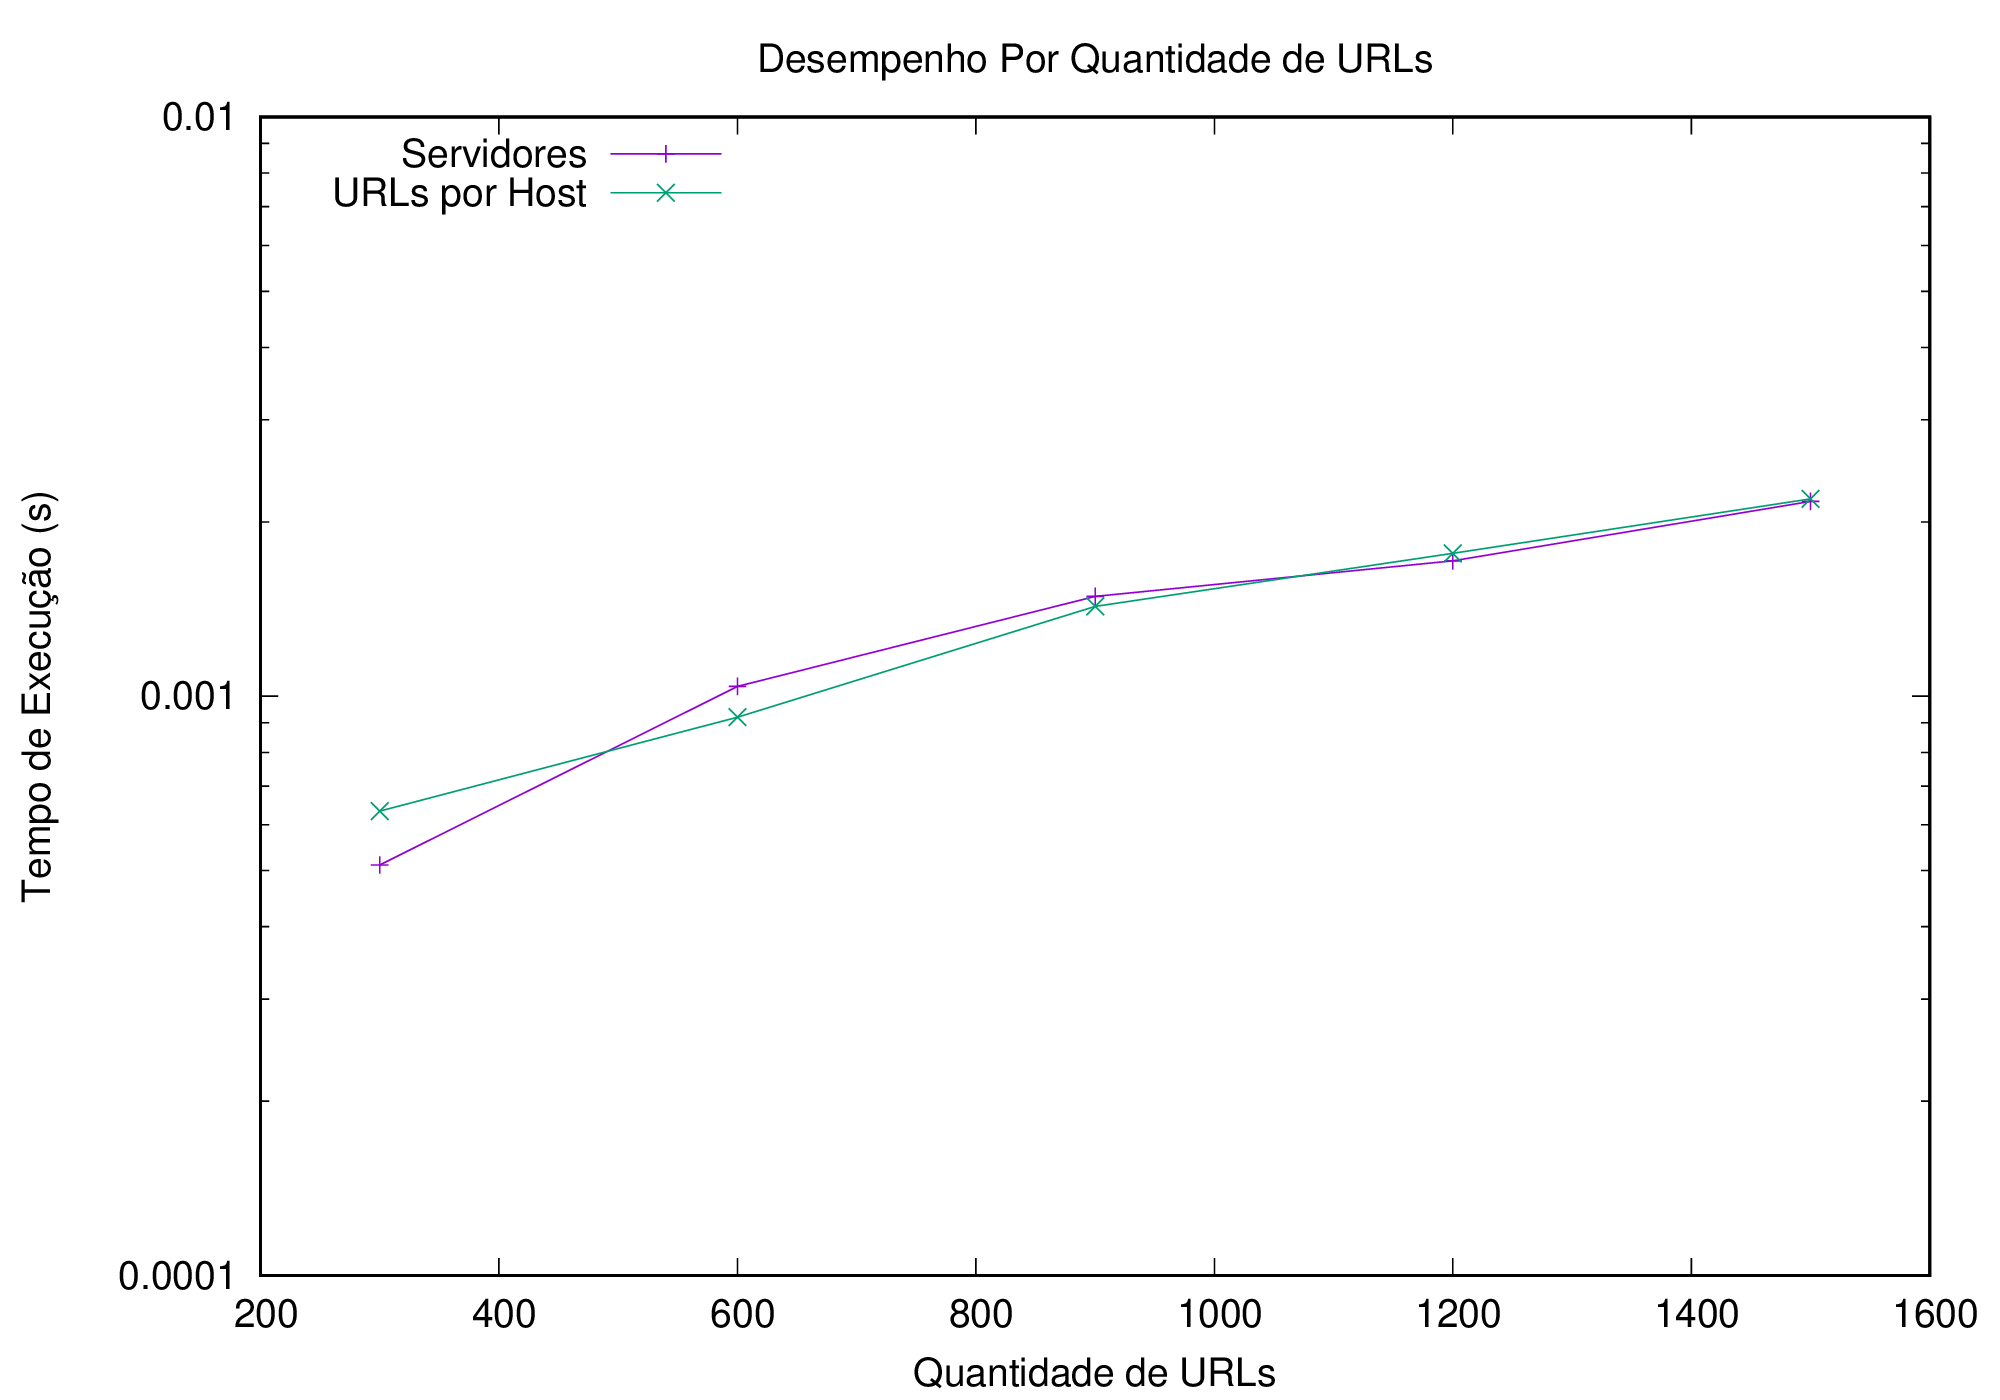
\includegraphics[width=10cm]{comp-perf.png} 
    \centering
\end{figure}

Mais especificamente, os parâmetros para o gerador de carga para o teste com servidores foram: \code{-s <quantidade> -u 3 -v 0 -p 5 -q 0.68}, em que a quantidade é a variável. A variança das URLs foi nula para se obter um número exato de URLs, e os parâmetros para a profundidade foram completamente arbitrários. Já no caso dos parâmetros para o teste variando as URLs por Host: \code{-s 30 -u <quantidade> -v 0 -p 5 -q 0.68}, em que a quantidade é a variável e as mesmas justificativas para os outros parâmetros se aplicam.

Os resultados obtidos não contradizem a análise de complexidade e estão dentro do esperado. Outro parâmetro analisado foi a \textit{profundidade} das URLs, mas não foi obtida diferença significativa para essa mudança (como esperado).

\subsection{Eficiência de Acesso à Memória}

\textit{Eu não consegui realizar essa análise.} 

Não por não tentar, mas eu realmente não consegui. Registrei parte dos meus esforços numa \textit{branch} no meu Github (cujo acesso pode ser solicitado). A minha proposta inicial era analisar somente a operação de escalonar tudo (e claro, as operações relacionadas, como a inserção e afins), registando o \textit{log} pelas células de URLs. E em algum momento até fiz algo convincente nesse sentido, o meu registro funcionava como esperado. No entanto, ao rodar o \code{analisamem}, o programa recebia um erro de segmentação, que eu não consegui depurar.

Tentei reduzir as operações de registro para evitar o \textit{segfault}, e é isso que a \textit{branch} contém. Apesar de ter conseguido \textit{esquivar} do segfault, o \code{analisamem} continuou não funcionando (parece que ele entra em um loop infinito, fazendo alto consumo de processamento).

\section{Conclusões}

Neste trabalho foi implementado um programa que é um componente de uma máquina de busca: um escalonador de URLs, usando a estratégia depth-first, fazendo uso de filas e listas alocadas dinamicamente e contando com leitura e escrita de arquivos.

\subsection{Aprendizado Pessoal}

Implementei, ainda que com grande ajuda, uma fila e uma lista encadeada. Como já tinha implementado uma pilha por causa de um dos exercícios das aulas, fico à mercê de implementar uma àrvore para completar as estruturas de dados básicas. Mas imagino que essas são cenas do próximo capítulo. Ainda sobre a implementação, uma coisa que pensei posteriormente é que talvez fosse mais interessante fazer uma implementação abstrata dessas classes e herdar, especificando as operações. 

Por exemplo, fazer uma lista encadeada genérica e criar uma classe lista encadeada de URLs, implementando as operações específicas de URLs. Isso seria muito interessante no sentido de que eu teria à minha disposição implementações prontas pra quando precisassse. Inclusive, acho que em algum momento, tentei fazer algo parecido, com templates, mas não foi muito pra frente. No geral, tive alguns problemas na hora de implementar essas estruturas, por causa da alocação dinâmica, mas no final evitei as condições que causavam erros.

Dessa vez, mal tive problemas com o \LaTeX, e até o momento em que estou escrevendo isso, não mexi com testes de unidade (mas usei um \textit{script} para rodar os testes disponibilizados). Usei \textit{branches} do \code{git} para gerenciar os desafios, mas isso não foi nada demais. Ou seja, meu ganho ``tangente'' não foi tão alto dessa vez.

Fazer as análises de complexidade foi mais uma vez bem trabalhoso. Fiquei meio chateado de ter \textit{comido uma mosca} no TP 0, mas a expectativa é que nesse devo ter comido \textit{mais}. Mas acho que estou começando a ganhar familiaridade com o assunto.

Eu estou desapontado por não ter conseguido fazer as análises de eficiência de acessoa à memória. Por outro lado, também acho que foi algo subespecificado (acho que faltou certo esforço em explicar isso). No mais, acredito que foi um bom trabalho, que teve suas dificuldades e aprendizados.

\section{Bibliografia}

\begin{enumerate}

    \item CHAIMOWICZ, Luiz. \textbf{Listas Encadeadas}. [S. l.], 24 ago. 2020. Disponível em: \url{https://www.youtube.com/watch?v=l4gEM46FznI}. Acesso em 6 dec 2021.

    \item CHAIMOWICZ, Luiz. \textbf{Filas - Implementação com Apontadores}. [S. l.], 24 ago. 2020. Disponível em: \url{https://www.youtube.com/watch?v=scNtNVD6HRE}. Acesso em 6 dec 2021.

\end{enumerate}


\newpage
\section*{Instruções}

\subsection*{Compilação}

Você pode compilar o programa da seguinte maneira:

\begin{enumerate}
    \item Utilize o comando \code{cd} para mudar de diretório para a localização da raiz do projeto;
    \item Utilize o comando \code{make}. 
\end{enumerate}

\subsection*{Execução}

Você pode rodar o programa da seguinte maneira:

\begin{enumerate}
    \item Utilize o comando \code{cd} para mudar de diretório para a localização da raiz do projeto;
    \item Utilize o comando \code{./bin/binary <nome-arquivo-entrada>}. Esse parâmetro é obrigatório!
\end{enumerate}

\end{document}
